%%%%%%%%%%%%%%%%%%%%%%%%%%%%%%%%%%%%%%%%%%%%%%%%
% chapter4.tex                                 %
% Contains formatting and content of chapter 4 %
%%%%%%%%%%%%%%%%%%%%%%%%%%%%%%%%%%%%%%%%%%%%%%%%
\chapter{Results}
\section{Numerical Results}

\begin{table}[H]
  \centering
  \begin{tabular}{@{}lllllll@{}}
  \toprule
  $\beta$ & $\Delta t_1$ & $\Delta t_{co}$ & $\Delta t_2$ & $J$ & $m_f/m_0$ & $m_f/m_{0h}$ \\ \midrule
  2 & 0.671 & 5.229 & 0.411 & 1.082 & 0.567062 & 0.56614 \\
  4 & 1.044 & 11.834 & 0.442 & 1.487 & 0.405365 & 0.407642 \\
  6 & 1.178 & 20.006 & 0.413 & 1.59 & 0.3638 & 0.368367 \\
  8 & 1.25 & 24.87 & 0.403 & 1.652 & 0.339164 & 0.353299 \\
  10 & 1.282 & 41.08 & 0.365 & 1.647 & 0.34106 & 0.346603 \\ \bottomrule
  \end{tabular}
  \end{table}

\begin{figure}[H]
    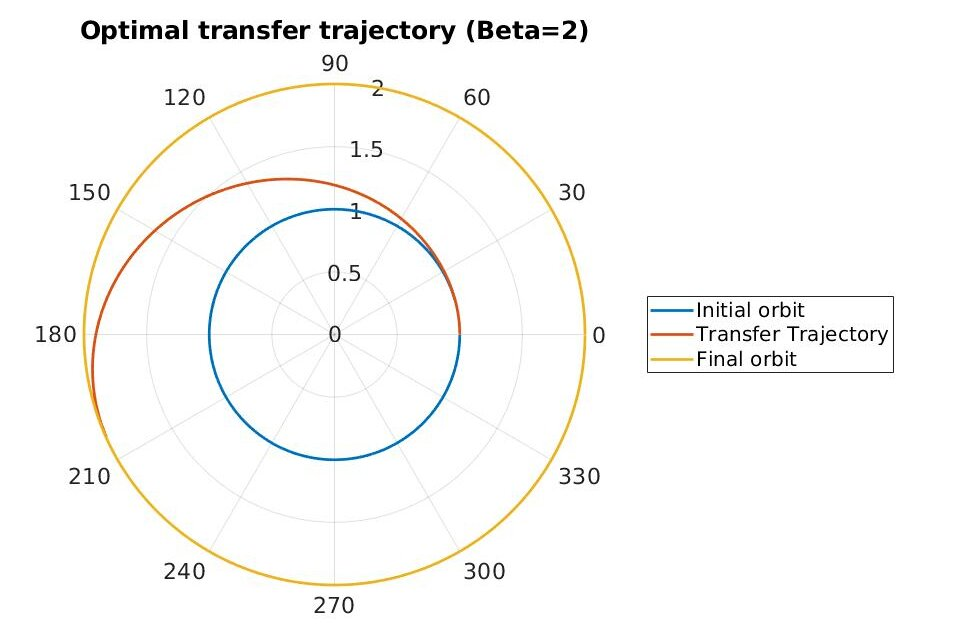
\includegraphics[width=\linewidth]{./jpgs/thrustArcB2.jpg}
    \caption{Numerically computed optimal transfer trajectory, $\beta = 2$.}
    \label{fig:Tarc-B2}
  \end{figure}


\begin{figure}[H]
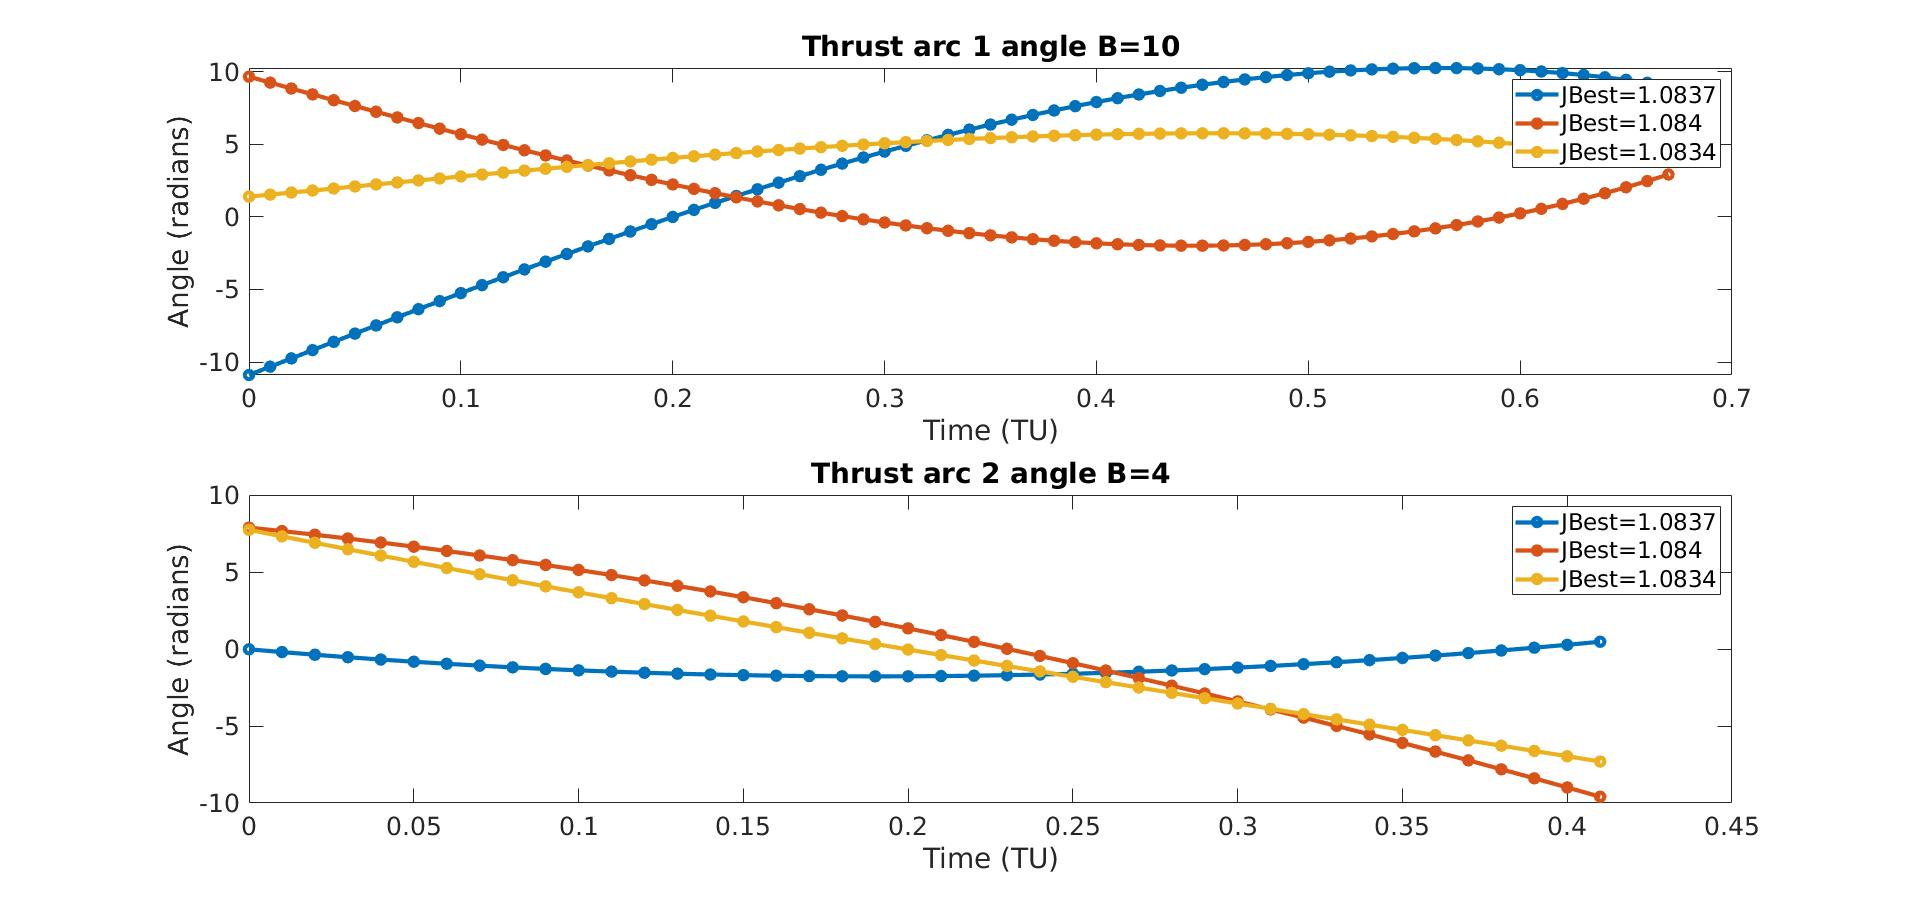
\includegraphics[width=\linewidth]{./jpgs/thrustAnglesB2.jpg}
\caption{Numerically computed thrust-angle time histories for optimal $\beta$ = 2 solutions  }

\end{figure}

\begin{figure}[H]
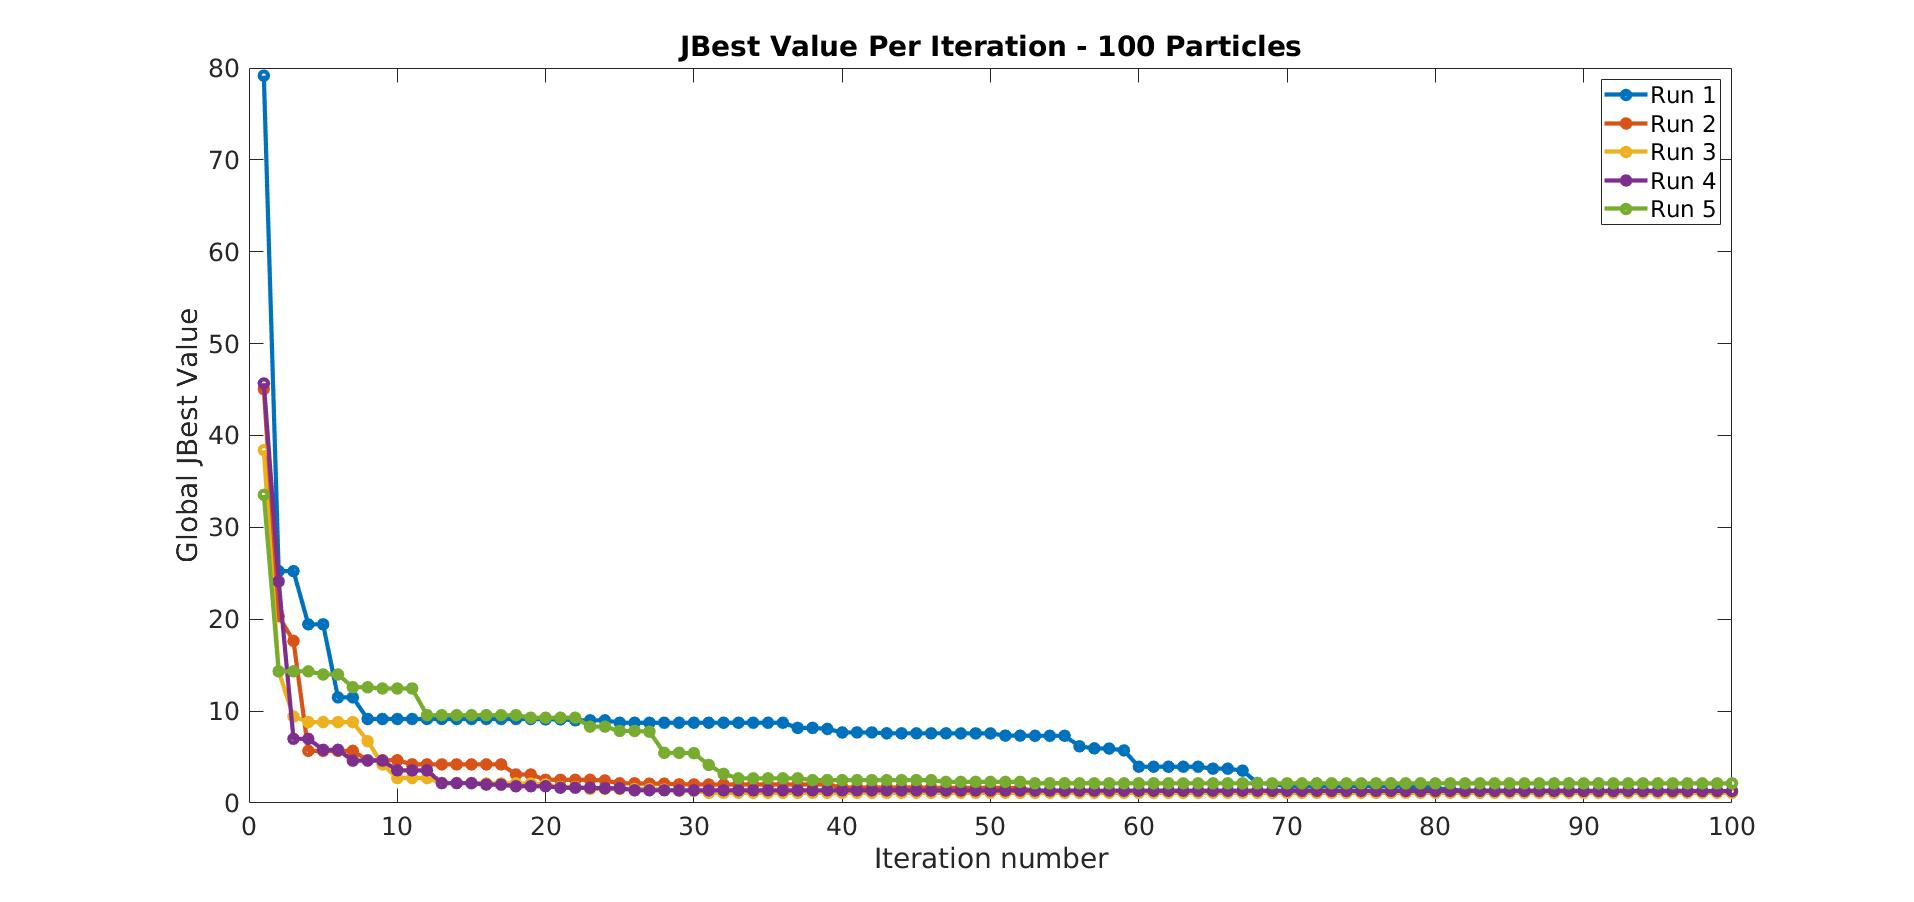
\includegraphics[width=\linewidth]{./jpgs/globalBestPerIteration100.jpg}
\caption{Global Best J Value Per Iteration: 100 Particles over 100 iterations}
\end{figure}


\begin{figure}[H]
    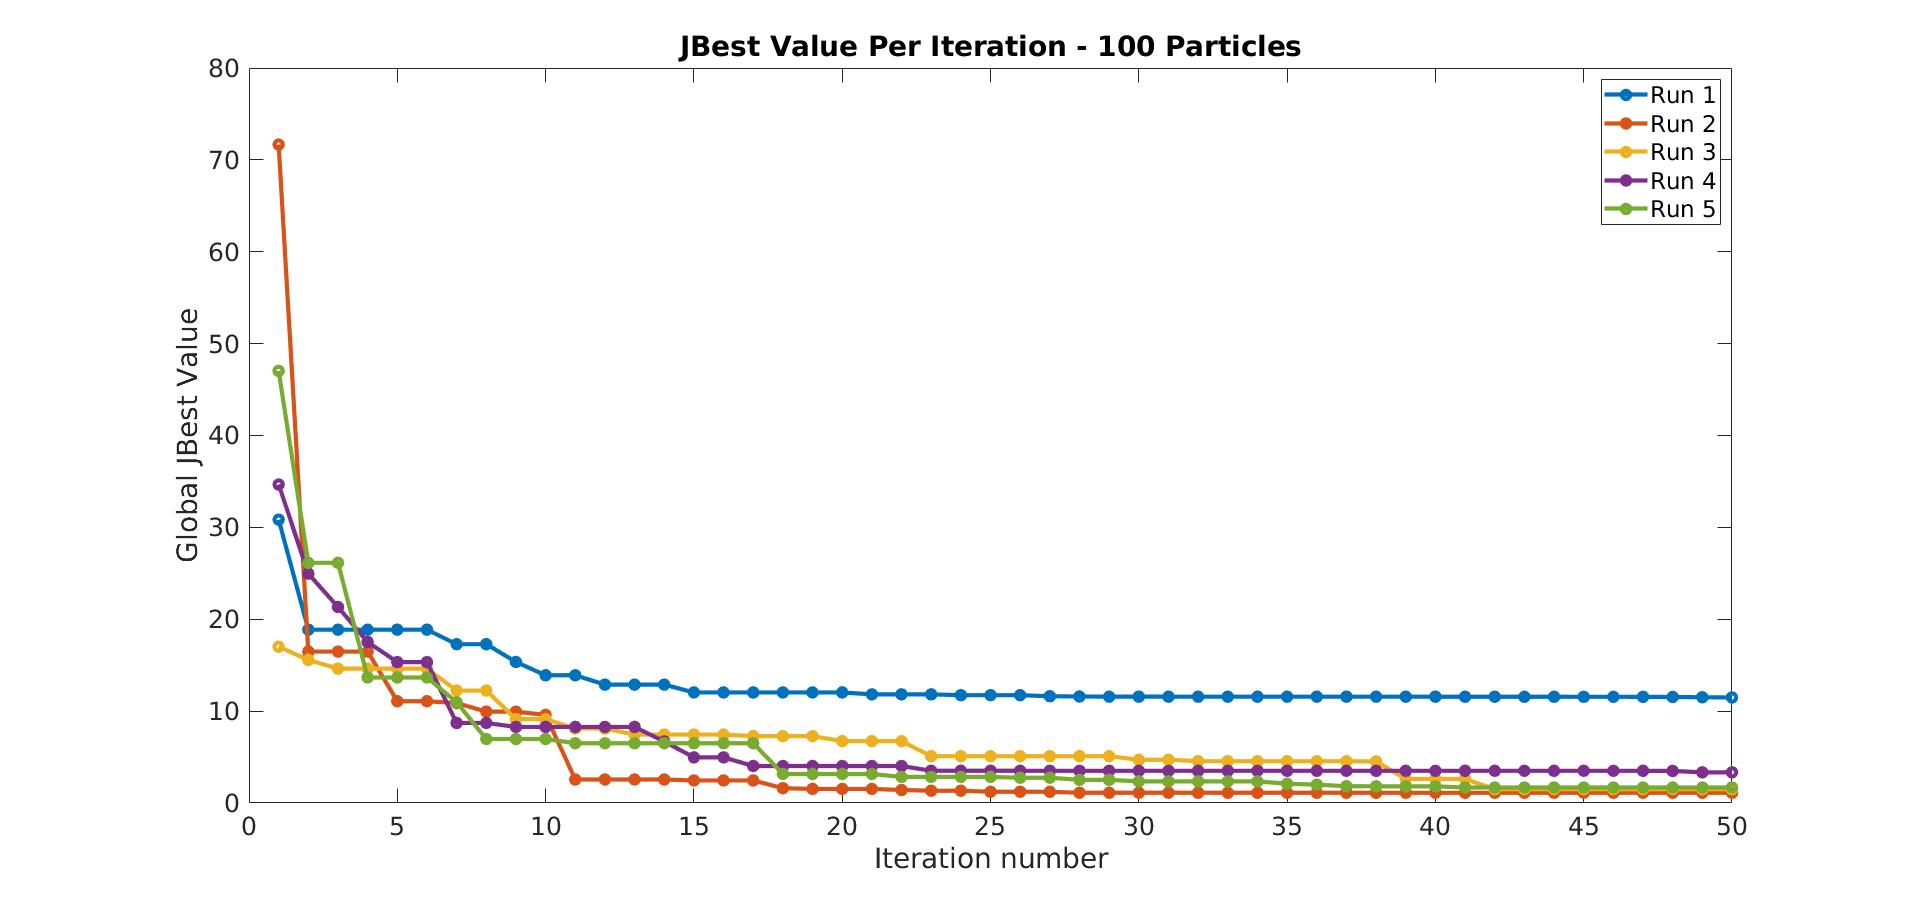
\includegraphics[width=\linewidth]{./jpgs/globalBestPerIteration50.jpg}
    \caption{Global Best J Value Per Iteration: 110 Particles over 100 iterations}
    \end{figure}


\begin{figure}[H]
    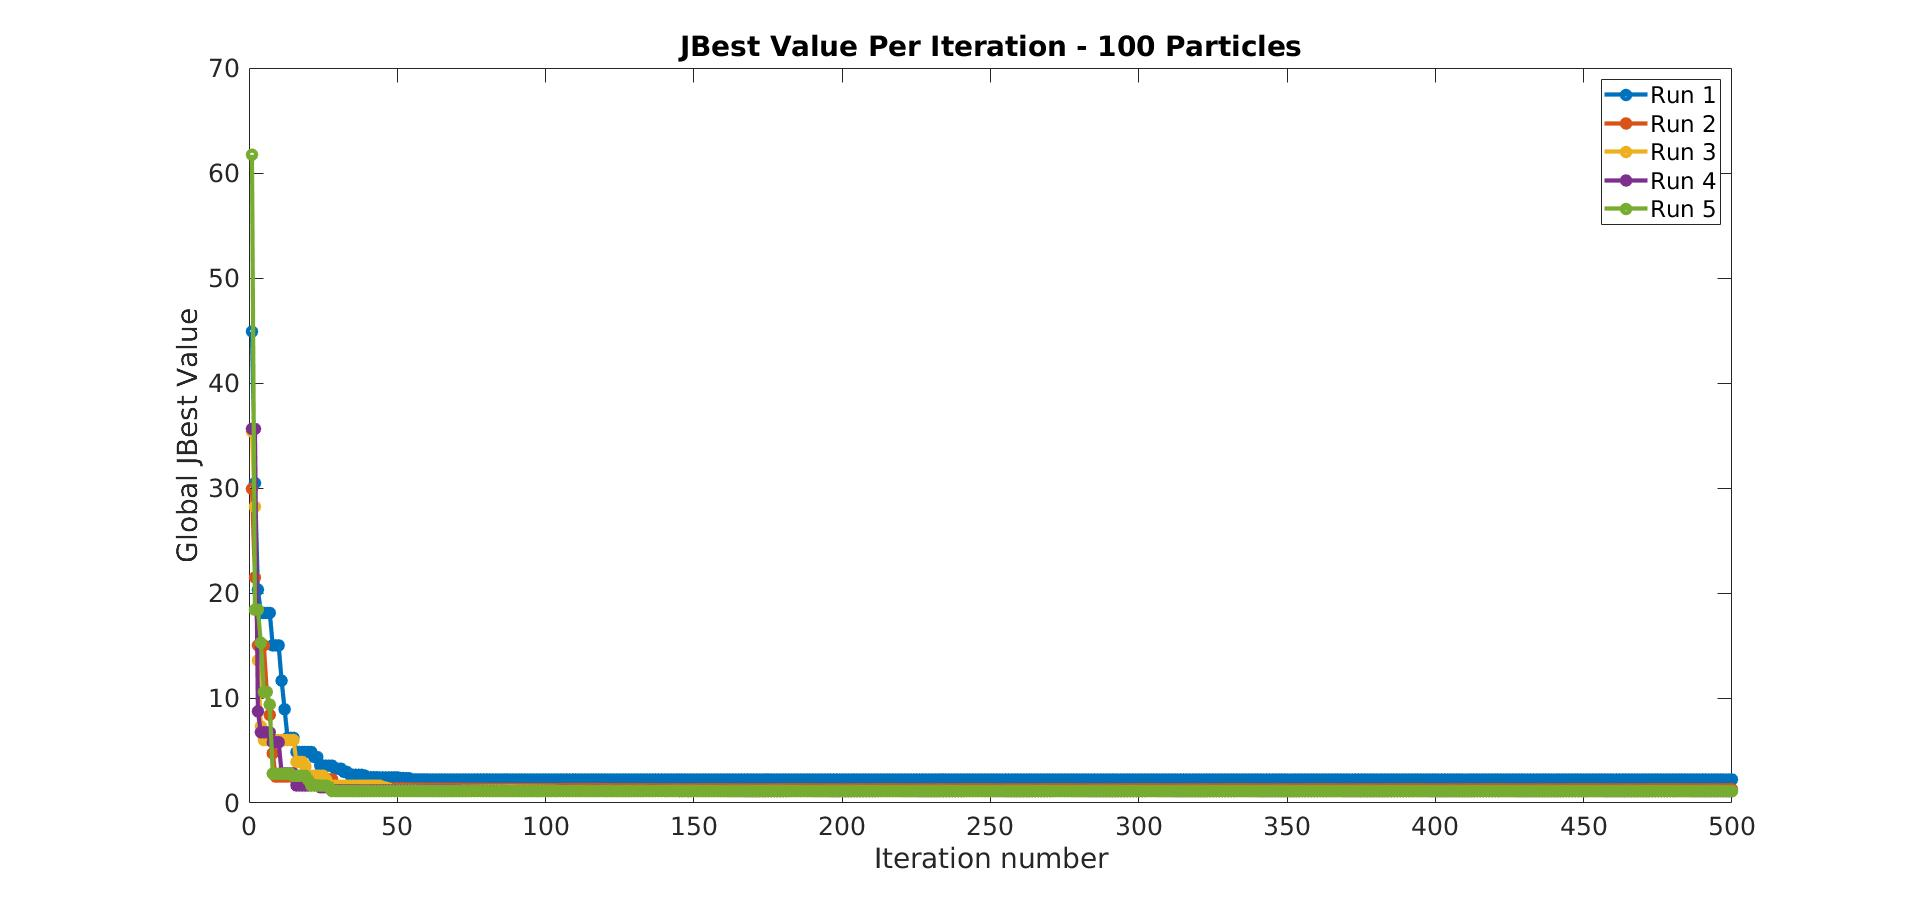
\includegraphics[width=\linewidth]{./jpgs/globalBestPerIteration500.jpg}
    \caption{Global Best J Value Per Iteration: 110 Particles over 500 iterations}
    \end{figure}
\section{Rehydration Results }

\begin{table}[H]
  \centering
  \begin{tabular}{lll|ll|ll}
    \toprule
    \multirow{2}{*}{25\% Rehydration} &
      \multicolumn{2}{c}{$\delta_{J}$ \textless .1\%} &
      \multicolumn{2}{c}{$\delta_{J}$ \textless 1\%} &
      \multicolumn{2}{c}{$\delta_{J}$ \textless 5\%} \\
      \cmidrule{2-7}
    & $J_{avg}$ & \% Change & $J_{avg}$ & \% Change & $J_{avg}$ & \% Change \\
    \midrule

    $n_{iter}=5$ & 1.347 & 44.177\% & 1.54 & 36.179\% & 1.438 & 40.406\% \\
    $n_{iter}=10$ & 1.421 & 41.11\% & 1.379 & 42.851\% & 1.594 & 33.941\% \\
    $n_{iter}=20$ & 1.331 & 44.840\% & 1.652 & 31.538\% & 1.503 & 37.712\% \\
    \bottomrule
  \end{tabular}
  \caption{Rehydration results for a 25\% population reset}
  \label{tab:rehydation-p25}
\end{table}

\begin{table}[H]
  \centering
  \begin{tabular}{lll|ll|ll}
    \toprule
    \multirow{2}{*}{33\% Rehydration} &
      \multicolumn{2}{c}{$\delta_{J}$ \textless .1\%} &
      \multicolumn{2}{c}{$\delta_{J}$ \textless 1\%} &
      \multicolumn{2}{c}{$\delta_{J}$ \textless 5\%} \\
      \cmidrule{2-7}
    & $J_{avg}$ & \% Change & $J_{avg}$ & \% Change & $J_{avg}$ & \% Change \\
    \midrule

    $n_{iter}=5$ & 1.371 & 43.18\% & 1.475 & 38.872\% & 1.412 & 41.484\% \\
    $n_{iter}=10$ & 1.364 & 43.47\% & 1.558 & 35.433\% & 1.473 & 40.448\% \\
    $n_{iter}=20$ & 1.412 & 41.48\% & 1.531 & 36.552\% & 1.578 & 34.604\% \\
    \bottomrule
  \end{tabular}
  \caption{Rehydration results for a 33\% population reset}
  \label{tab:rehydation-p33}
\end{table}


\begin{table}[H]
    \centering
    \begin{tabular}{lll|ll|ll}
      \toprule
      \multirow{2}{*}{50\% Rehydration} &
        \multicolumn{2}{c}{$\delta_{J}$ \textless .1\%} &
        \multicolumn{2}{c}{$\delta_{J}$ \textless 1\%} &
        \multicolumn{2}{c}{$\delta_{J}$ \textless 5\%} \\
        \cmidrule{2-7}
      & $J_{avg}$ & \% Change & $J_{avg}$ & \% Change & $J_{avg}$ & \% Change \\
      \midrule

      $n_{iter}=5$ & 1.58 & 34.52\% & 1.469 & 39.12\% & 1.425 & 40.94\% \\
      $n_{iter}=10$ & 1.396 & 42.15\% & 1.306 & 45.88\% & 1.473 & 38.96\% \\
      $n_{iter}=20$ & 1.373 & 43.10\% & 1.39 & 42.40\% & 1.33 & 44.88\% \\
      \bottomrule
    \end{tabular}
    \caption{Rehydration results for a 50\% population reset}
    \label{tab:rehydation-p50}
  \end{table}

\section{Speedup}

\subsection{MATLAB}

%Putting the H here ensures the table goes exactly where you put
%it in the code
\begin{table}[H]
    \centering
    \begin{tabular}{@{}llll@{}}
    \toprule
    \textbf{Num Particles} & \textbf{Num Particles} & \textbf{Num Iterations} & \textbf{Time (s)} \\ \midrule
    25            & 25            & 250            & 30.527   \\
    25            & 25            & 500            & 39.15    \\
    25            & 25            & 1000           & 68.88    \\
    50            & 50            & 250            & 30.527   \\
    50            & 50            & 500            & 80.4246  \\
    50            & 50            & 1000           & 141.151  \\
    100           & 100           & 250            & 95.956   \\
    100           & 100           & 500            & 152.22   \\
    100           & 100           & 1000           & 306.732  \\
    150           & 150           & 250            & 161.3    \\
    150           & 150           & 500            & 195.87   \\
    150           & 150           & 1000           & 388.03   \\
    200           & 200           & 250            & 157.061  \\
    200           & 200           & 500            & 251.575  \\
    200           & 200           & 1000           & 457.55   \\ \bottomrule
    \end{tabular}
    \caption{MATLAB Numerical Results - Wall Clock Time}
    \label{tab:MATLAB-speedup}
    \end{table}

\subsection{C++ Single Threaded}

% Please add the following required packages to your document preamble:
% \usepackage{booktabs}
\begin{table}[H]
    \centering
    \begin{tabular}{@{}llll@{}}
    \toprule
    \textbf{Num Particles} & \textbf{Time (s)} & \textbf{\% Speedup to MATLAB} & \textbf{X faster than MATLAB} \\ \midrule
    25            & 1.732    & 94.32633406          & 17.62528868              \\
    25            & 2.39     & 93.89527458          & 16.38075314              \\
    25            & 3.92     & 94.30894309          & 17.57142857              \\
    50            & 2.96     & 90.30366561          & 10.31317568              \\
    50            & 3.26     & 95.94651388          & 24.6701227               \\
    50            & 5.695    & 95.96531374          & 24.78507463              \\
    100           & 6.659    & 93.060361            & 14.40997147              \\
    100           & 7.21     & 95.2634345           & 21.11234397              \\
    100           & 11.83    & 96.14321297          & 25.92831784              \\
    150           & 7.26     & 95.49907006          & 22.21763085              \\
    150           & 12.64    & 93.54674018          & 15.4960443               \\
    150           & 16.68    & 95.7013633           & 23.26318945              \\
    200           & 7.77     & 95.05287754          & 20.21377091              \\
    200           & 11.423   & 95.45940574          & 22.02354898              \\
    200           & 21.06    & 95.39722435          & 21.72602089              \\ \bottomrule
    \end{tabular}
    \caption{C++ Single Threaded Speedup Results - Wall Clock Time}
    \label{tab:ST-speedup}
    \end{table}


\subsection{C++ OpenMP}
\begin{table}[H]
    \centering
    \begin{tabular}{@{}lllll@{}}
    \toprule
    \textbf{Num Particles} & \textbf{Time (s)} & \textbf{\% Speedup: MATLAB} & \textbf{\% Speedup: 1 Thread} & \textbf{X faster than MATLAB} \\ \midrule
    25  & 1.78  & 94.16909621 & -2.771362587 & 17.15       \\
    25  & 3.4   & 91.31545338 & -42.25941423 & 11.51470588 \\
    25  & 5.23  & 92.40708479 & -33.41836735 & 13.17017208 \\
    50  & 2.81  & 90.7950339  & 5.067567568  & 10.86370107 \\
    50  & 4.77  & 94.06897889 & -46.3190184  & 16.86050314 \\
    50  & 8.51  & 93.9709956  & -49.42932397 & 16.58648649 \\
    100 & 5.71  & 94.04935595 & 14.2513891   & 16.80490368 \\
    100 & 6.6   & 95.66417028 & 8.460471567  & 23.06363636 \\
    100 & 11.73 & 96.17581472 & 0.8453085376 & 26.14936061 \\
    150 & 4.92  & 96.94978301 & 32.23140496  & 32.78455285 \\
    150 & 9.77  & 95.01199775 & 22.7056962   & 20.04810645 \\
    150 & 13.93 & 96.41007139 & 16.48681055  & 27.85570711 \\
    200 & 5.88  & 96.25623166 & 24.32432432  & 26.71105442 \\
    200 & 10.46 & 95.84219418 & 8.4303598    & 24.05114723 \\
    200 & 22.42 & 95.09998907 & -6.457739791 & 20.40811775 \\ \bottomrule
    \end{tabular}
    \caption{OpenMP Speedup Results - Wall Clock Execution Time}
    \label{tab:OpenMP-speedup}
    \end{table}

\newpage